% Chapter 1

\chapter{Introducción General} % Main chapter title

\label{Chapter1} % For referencing the chapter elsewhere, use \ref{Chapter1} 
\label{IntroGeneral}

En este capítulo se verá una breve introdución al proceso de elaboración del vino, mencionaremos cual fue motivación por la cual se realizó este proyecto y en que consiste el proyecto CIAA. 

%----------------------------------------------------------------------------------------

% Define some commands to keep the formatting separated from the content 
\newcommand{\keyword}[1]{\textbf{#1}}
\newcommand{\tabhead}[1]{\textbf{#1}}
\newcommand{\code}[1]{\texttt{#1}}
\newcommand{\file}[1]{\texttt{\bfseries#1}}
\newcommand{\option}[1]{\texttt{\itshape#1}}
\newcommand{\grados}{$^{\circ}$}

%----------------------------------------------------------------------------------------

\section{Introducción}

%----------------------------------------------------------------------------------------

\section{Proceso de elaboración del vino}
Si bien el proceso de elaboración del vino se fue perfeccionando y se ha vuelta muy complejo pero la esencia sigue siendo la misma.
Las partes del proceso se dividen en:

\begin{description}
  \item[La vendimia o cosecha:] este consiste en la recolección de la uva, la cual en Argentina se suele realizar entre los meses de Febrero y Abril.
  \item[Pesada:] En esta etapa se pesa la uva de la variedad como Cabernet Sauvignon, Malbec, Syrah, Merlot y Tempranilla.
  \item[Despalillado:] es el proceso mediante el cual se separa la uva del resto del racimo.
  \item[Estrujado:] Desgranado el racimo, las uvas se pasan por una pisadora para conseguir que se rompa la piel de la uva, llamada hollejo. Así se extrae el mosto para facilitar el siguiente paso, pero no se debe estrujar demasiado para evitar que se rompan las semillas de las uvas. Las semillas serán eliminadas.
  \item[Fermentación:] El mosto ingresa a los tanques de acero inoxidable junto al hollejo y allí comienza el proceso de fermentación a una temperatura de 20-24ºC durante 6-8 días.
  \item[Descube:] En este proceso se separan el hollejo del vino, mediante bombas. El hollejo sufre una prensada y si el vino obtenido es de baja calidad sigue un proceso distinto y si la calidad es buena es agregado al vino obtenido por fermentación, continuando su mismo proceso de vinificación.
  \item[Primer trasiego:] Se eliminan las levaduras y otros tipos de sedimentos, mediante bombas y de un tanque a otro.
  \item[Segundo trasiego:] El vino es conducido a otro tanque para hacer el segundo trasiego por medio de bombas. El segundo trasiego se efectúa para separar las borras más finas y las levaduras que pueden haber quedado en el vino.
  \item[Clarificado:] Se realza en otro tanque de acero inoxidable con bombas y con bentonita. Aquí se purifica el vino durante 24-48-72 horas. Después se realiza un trasiego para eliminar la bentonita.
  \item[Filtrado:] Aquí se limpia el vino mediante filtradores y con el agregado de tierras filtrantes. Posteriormente, se hacen trasiegos para eliminar los restos de tierras filtrantes.
  \item[Fraccionado:] El vino de los tanques es transportado mediante bombas hacia la sala de fraccionamiento donde se llenan las botellas, se tapan, se etiquetan y se acomodan en cajas para ser comercializadas.
\end{description}

Se aprecia el esquema de elaboración del vino en la figura \ref{fig:winep}.

\begin{figure}[hp]
  \centering
  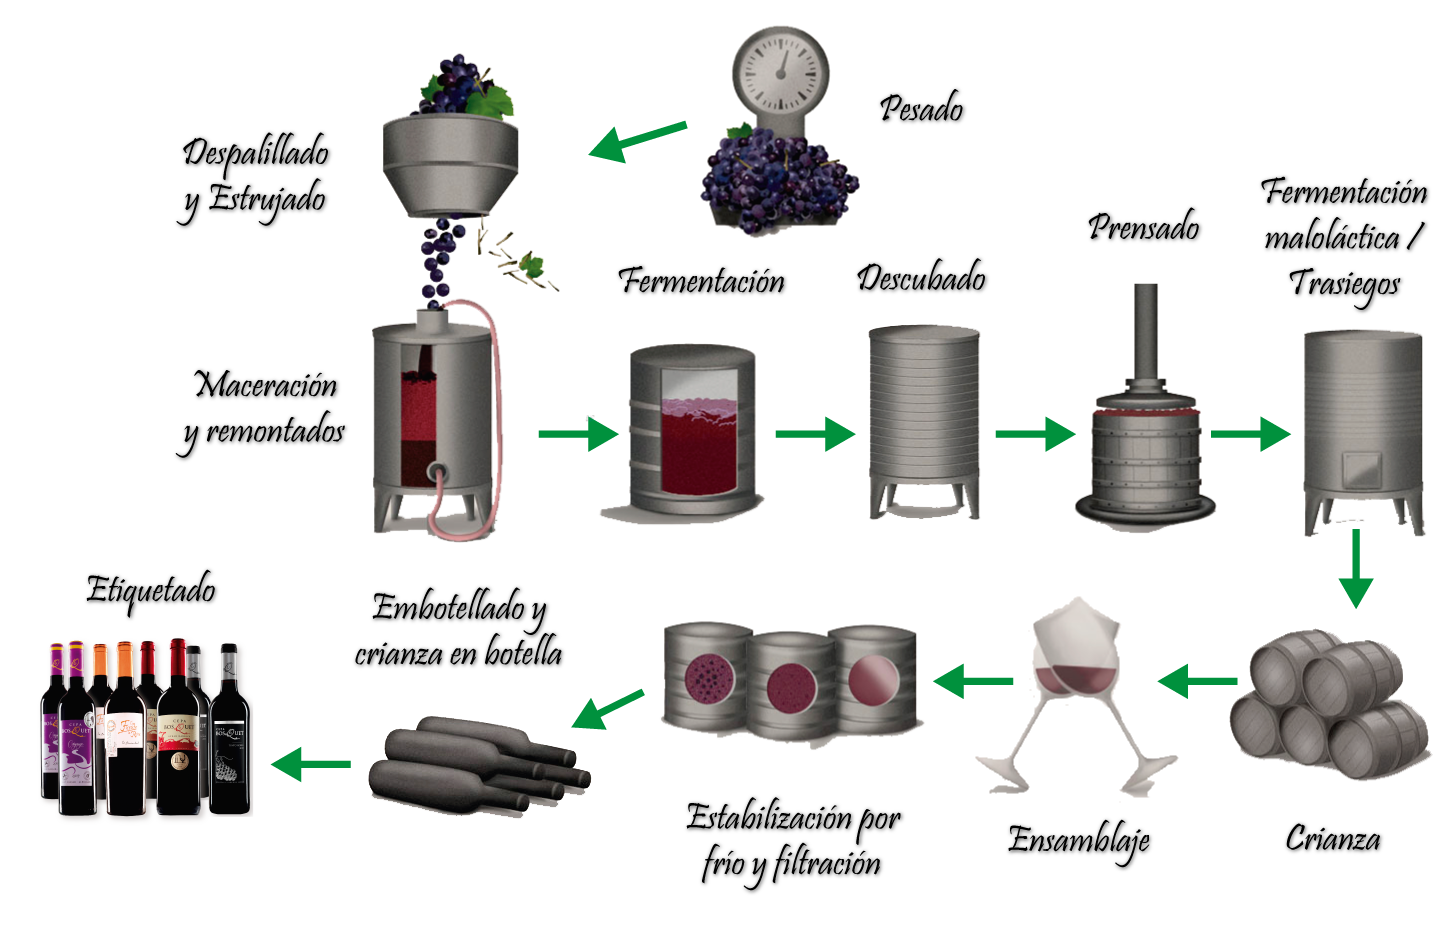
\includegraphics[scale=.3]{./Figures/elaboracion-del-vino-tinto.png}
  \caption{Esquema de elaboracirón de vino tinto.}
  \label{fig:winep}
\end{figure}


\subsection{La temperatura}

  Un factor vital para que la fermentación siga correctamente su curso. Es importante saber que, si la temperatura de fermentación es elevada, esos grados de más matarán prematuramente las levaduras (que no podrán completar su función metabólica).

  Pero, además de este aspecto de vital importancia, también es necesario saber que una temperatura excesiva provocará la pérdida de elementos aromáticos y un incremento del amargor (ya que el calor puede desencadenar una reacción química de las partes sólidas procedentes de la vid, como pueden ser los hollejos).

  Por este motivo, la temperatura es uno de los aspectos más vigilados en el proceso de fermentación del vino incluso desde antes de dejar que la naturaleza obre sus misterios químicos


\section{Motivación}

En el presente trabajo se busca satisfacer las necesidades de la bodega de mi primo. La cual se necesita controlar un proceso delicado como es la fermentación del vino y se requiere un cuidado continúo. Por el momento es realizado por personal día y noche. Teniendo en cuenta que en la zona de trabajo es difícil conseguir personas responsables que se comprometan con el trabajo. 

A su vez se busca también una satisfacción personal, dado que hacía tiempo que quería poder implementar en un microcontrolador una interfaz que permita visualizar la información de un sistema mediante una plataforma web, donde se pueda apreciar el estado de las entradas y poder ejercer control sobre ellas.

Y para concluir, el hecho de utilizar la plataforma CIAA, la cual me permitió cumplir todo estos objetivos personales, haciendo uso de un sistema operativo de tiempo real (RTOS), como sé llamará de aquí en adelante.



\section{Proyecto CIAA}

El Proyecto CIAA cuyas siglas hacen referencia a Computadora Industrial Abierta Argentina, nació en 2013 como una iniciativa conjunta entre el sector académico y el industrial, representados por la ACSE\footnote{Asociación Civil para la investigación, promoción y desarrollo de los Sistemas electrónicos Embebidos.} y CADIEEL\footnote{Cámara Argentina de Industrias Electrónicas, Electromecánicas y Luminotécnicas.}, respectivamente \citep{CIAA}.

\subsection{Objetivos del proyecto}
\begin{enumerate}
  \item Impulsar el desarrollo tecnológico nacional, a partir de sumar valor agregado al trabajo y a los productos y servicios, mediante el uso de sistemas electrónicos, en el marco de la vinculación de las instituciones educativas y el sistema científico-tecnológico con la industria.
  \item Darle visibilidad positiva a la electrónica argentina.
  \item Generar cambios estructurales en la forma en la que se desarrollan y utilizan en nuestro país los conocimientos en el ámbito de la electrónica y de las instituciones y empresas que hacen uso de ella.
\end{enumerate}

Es importante destacar que La CIAA-NXP es la primera y única computadora del mundo que reúne dos cualidades:

\begin{enumerate}
  \item Ser Industrial, ya que su diseño está preparado para las exigencias de confiabilidad, temperatura, vibraciones, ruido electromagnético, tensiones, cortocircuitos, etc., que demandan los productos y procesos industriales.
  \item Ser Abierta, ya que toda la información sobre su diseño de hardware, firmware, software, etc. está libremente disponible en internet bajo la Licencia BSD, para que cualquiera la utilice como quiera.
\end{enumerate}

\subsection{¿Qué es la CIAA-NXP?}

La CIAA-NXP es la primer CIAA en ser diseñada, probada y producida en serie. Se puede apreciar en la figura \ref{fig:ciaaxp}. Pensada para utilizarse en (pero no limitada a) equipos de automatización industrial. Se alimenta con 24V (CC). Tiene entradas digitales optoacopladas, entradas analógicas configurables 0-10V o 0-20mA, salidas digitales open-drain y relé, salida analógica configurable 0-10V o 0-20mA, interfaces de comunicación RS232, RS485, CAN, Ethernet y USB-OTG. Basada en el microcontrolador LPC4337. 

\begin{figure}[ht]
  \centering
  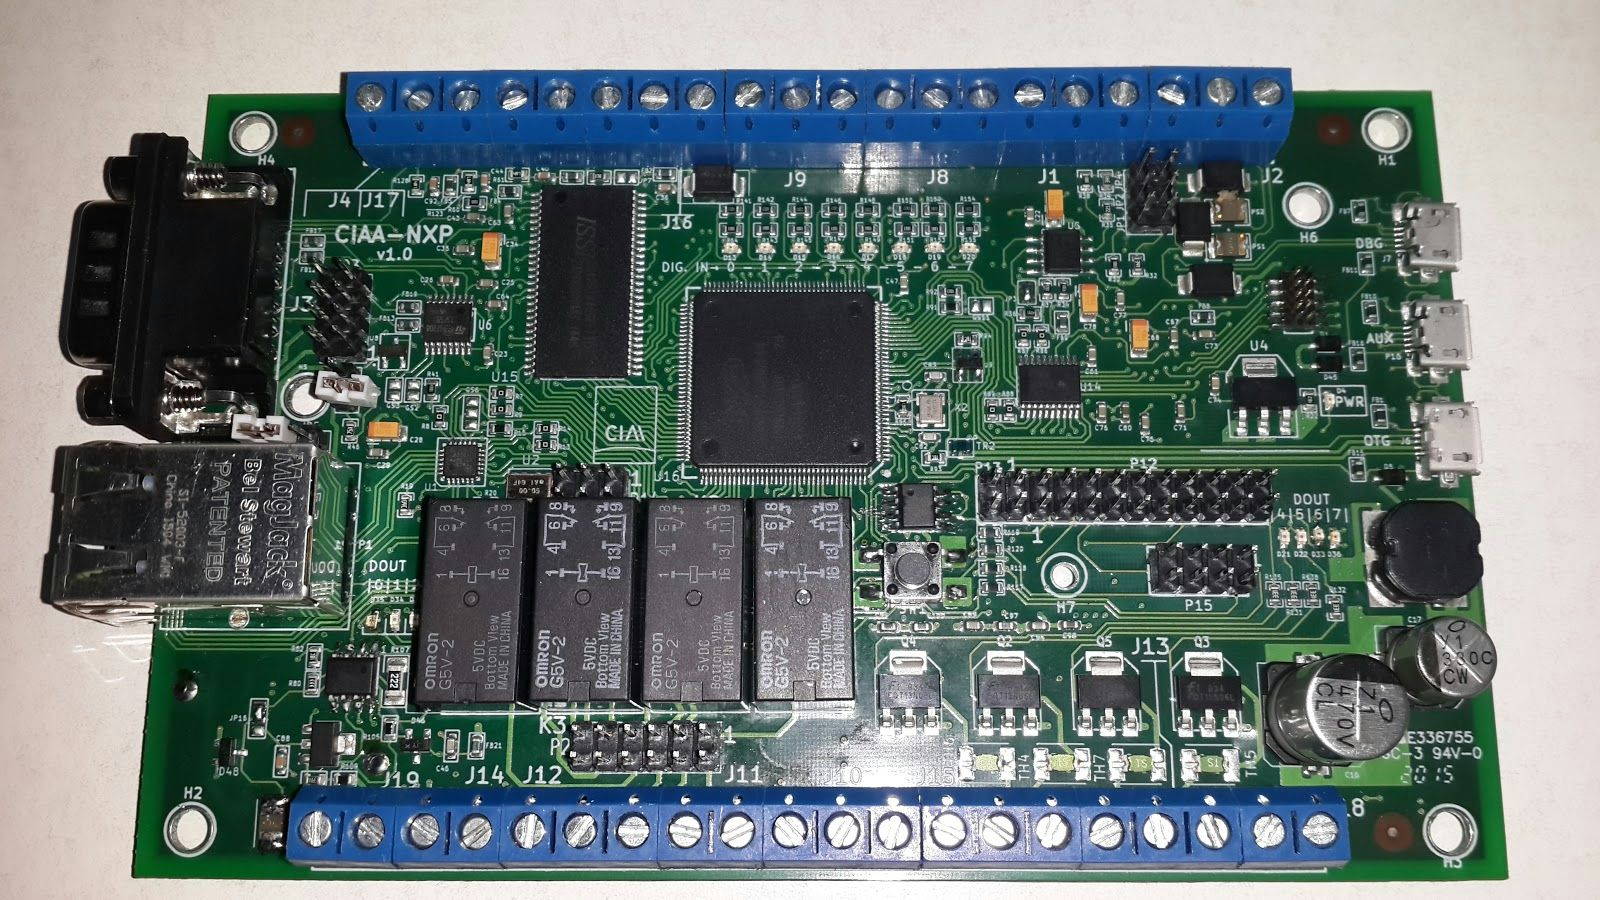
\includegraphics[scale=.2]{./Figures/ciaa.png}
  \caption{Placa CIAA-NXP para la industria.}
  \label{fig:ciaaxp}
\end{figure}

La especificaciones CIAA-NXP son :
\begin{description}
  \item[CPU:] Microcontrolador LPC4337JDB144\footnote{\url{http://www.nxp.com/products/microcontrollers/cortex_m4/lpc4300/LPC4337JBD144.html}}. Dual-core Cortex-M4 + Cortex-M0 @ 204MHz.
  \item[Debuger:] USB-to-JTAG FT2232H\footnote{\url{http://www.ftdichip.com/Support/Documents/DataSheets/ICs/DS_FT2232H.pdf}}. Soportado por OpenOCD.

  \item[Memorias:]
  \hspace{1cm}
  \begin{itemize}
      \item Memorias internas del LPC4337. Ver Hoja de datos del LPC4337JBD144
      \item SDRAM 128 Mbit (IS42S16800F-7TL o compatible)
      \item Flash QSPI 32 Mbit (S25FL032P0XMFI011 o compatible)
      \item EEPROM 1 Mbit y 2 Kbit
    \end{itemize}
  \item[Interfaces de comunicación:] 
  \hspace{1cm}
    \begin{itemize}
      \item Ethernet con soporte PoE.
      \item USB On-The-Go.
      \item USB Device Auxiliar.
      \item RS232 (detalles técnicos).
      \item RS485.
      \item CAN (detalles técnicos).
    \end{itemize}
  \item[Entradas/Salidas:] 
  \hspace{1cm}
    \begin{itemize}
      \item 8 entradas digitales optoacopladas.
      \item 4 entradas analógicas configurables por jumper 0-10V o 0-20mA.
      \item 4 salidas open-drain de 24V, 1A.
      \item 4 salidas a relé 24V, 2A.
      \item 1 salida analógica configurable por jumper 0-10V o 0-20mA.
      \item Conectores de expansión LV-GPIO, SPI, I2C.
    \end{itemize}
\end{description}


